\documentclass[12pt,a4paper]{article}

\setcounter{section}{0}

\usepackage[utf8]{inputenc}
\usepackage[english]{babel}
\usepackage{amssymb, amsmath}
\usepackage{fullpage}
\usepackage{parskip}
\usepackage{url}
\usepackage{color}
\usepackage{enumitem}
\usepackage{graphicx}

\graphicspath{{../OUTPUT/}}

\newcommand{\from}{\colon}
\newcommand{\norm}[1]{\left\|#1\right\|}

\begin{document}
    
    %%%%%%%%%%%%%%%%%%%%%%%%%%%%%%%%%%%%%%%%%%%%%%%%%%
    Bolt -- homework \hfill R.A., \today
    %%%%%%%%%%%%%%%%%%%%%%%%%%%%%%%%%%%%%%%%%%%%%%%%%%
    
    
    %%%%%%%%%%%%%%%%%%%%%%%%%%%%%%%%%%%%%%%%%%%%%%%%%%
    \section{Most undersupplied hours}
    %%%%%%%%%%%%%%%%%%%%%%%%%%%%%%%%%%%%%%%%%%%%%%%%%%
    
    As an indicator of most undersupplied hours,
    it makes sense to take
    the hours where
    most people did not see an available car
    in the app,
    as found in the \emph{demand data} table.
    %
    Weekly averages look as follows:
    
    \begin{center}
        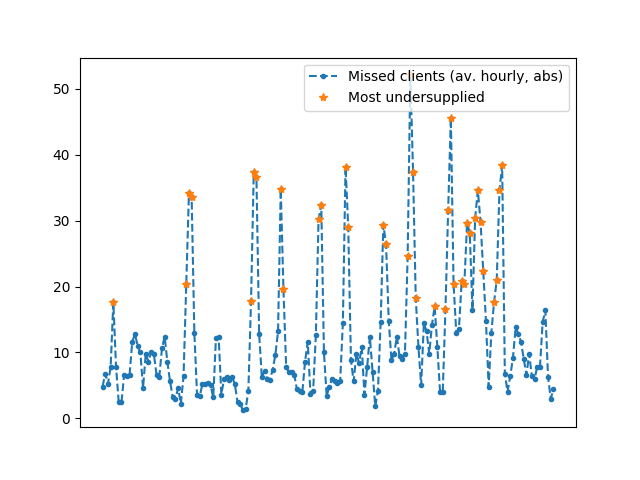
\includegraphics[width=0.7\textwidth]{task1/undersupp_abs}
    \end{center}
    
    The peaks are (in order of decreasing undersuppy):
    Thu--18,
    Fri--09,
    Sat--04,
    Wed--18,
    Thu--19,
    Tue--08,
    Tue--09,
    Tue--18,
    Sat--03,
    Fri--19,
    Mon--08,
    Mon--09,
    Wed--09,
    Fri--08,
    Fri--18,
    Wed--08,
    Fri--20,
    Fri--15,
    Thu--08,
    Wed--19,
    Fri--16,
    Thu--09,
    Thu--17,
    Fri--21,
    Sat--02,
    Fri--13,
    Mon--07,
    Fri--10,
    Fri--14,
    Tue--19,
    Thu--20,
    Tue--07,
    Sat--01,
    Sun--04,
    Fri--03,
    Fri--07.
    
    \newpage
    
    %%%%%%%%%%%%%%%%%%%%%%%%%%%%%%%%%%%%%%%%%%%%%%%%%%
    \section{24h curve of average supply and demand}
    %%%%%%%%%%%%%%%%%%%%%%%%%%%%%%%%%%%%%%%%%%%%%%%%%%

    By ``supply'' we mean number of people who saw a car
    and by ``demand'' we mean also those that did not,
    as found in the \emph{demand data} table.
    
    \begin{center}
        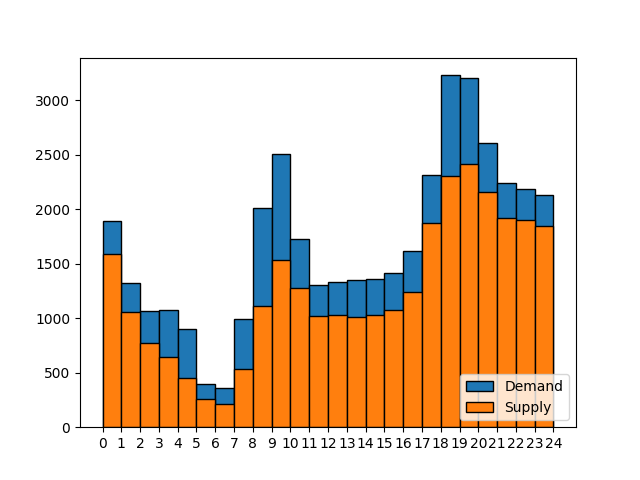
\includegraphics[width=0.8\textwidth]{task2/supply-demand}
    \end{center}

    
    
    %%%%%%%%%%%%%%%%%%%%%%%%%%%%%%%%%%%%%%%%%%%%%%%%%%
    \section{Visualisation of hours of undersupply}
    %%%%%%%%%%%%%%%%%%%%%%%%%%%%%%%%%%%%%%%%%%%%%%%%%%
    
    
    \begin{center}
        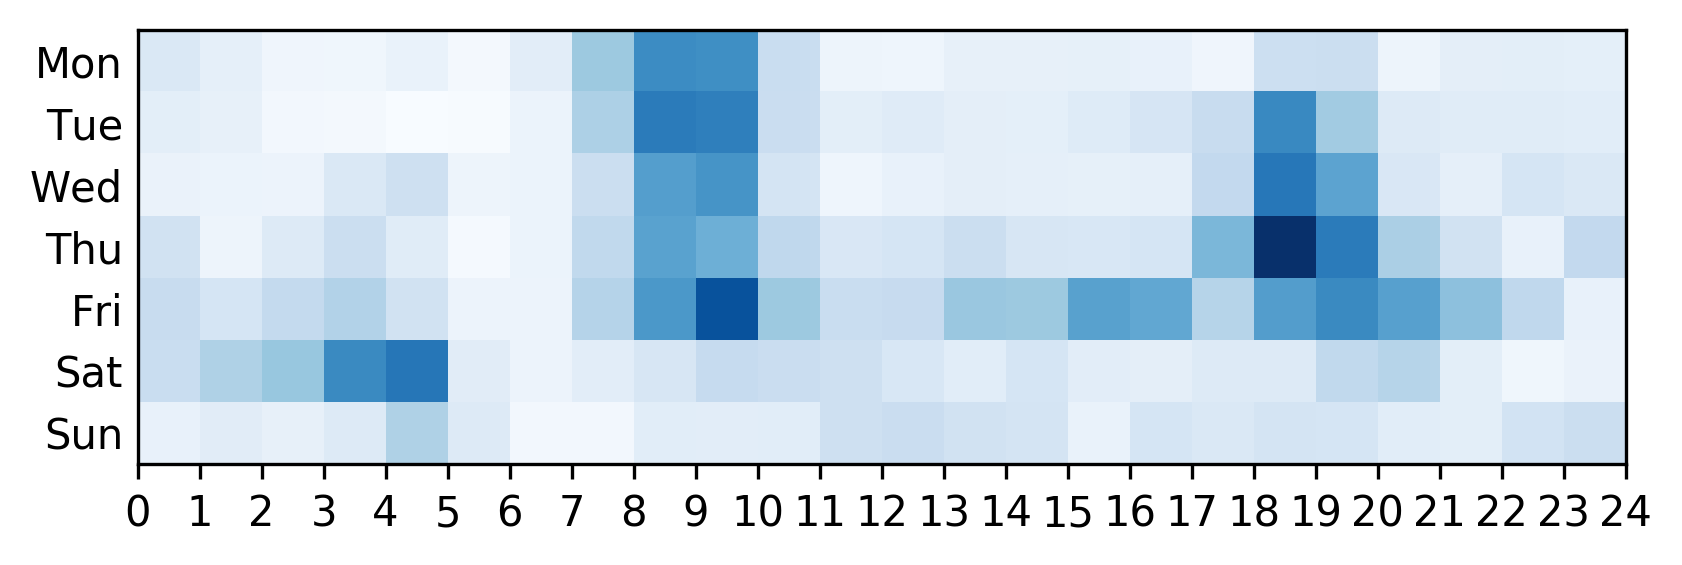
\includegraphics[width=1\textwidth]{task3/undersupp_heat}
    \end{center}
    
    
    %%%%%%%%%%%%%%%%%%%%%%%%%%%%%%%%%%%%%%%%%%%%%%%%%%
    \section{Number of hours for high Coverage Ratio}
    %%%%%%%%%%%%%%%%%%%%%%%%%%%%%%%%%%%%%%%%%%%%%%%%%%
    
    Estimate extra hours needed 
    \begin{align}
        \text{online hours} \times
        \frac{\text{people saw no car}}{\text{people saw a car}}
        .
    \end{align}

    This results in the following image
    \begin{center}
        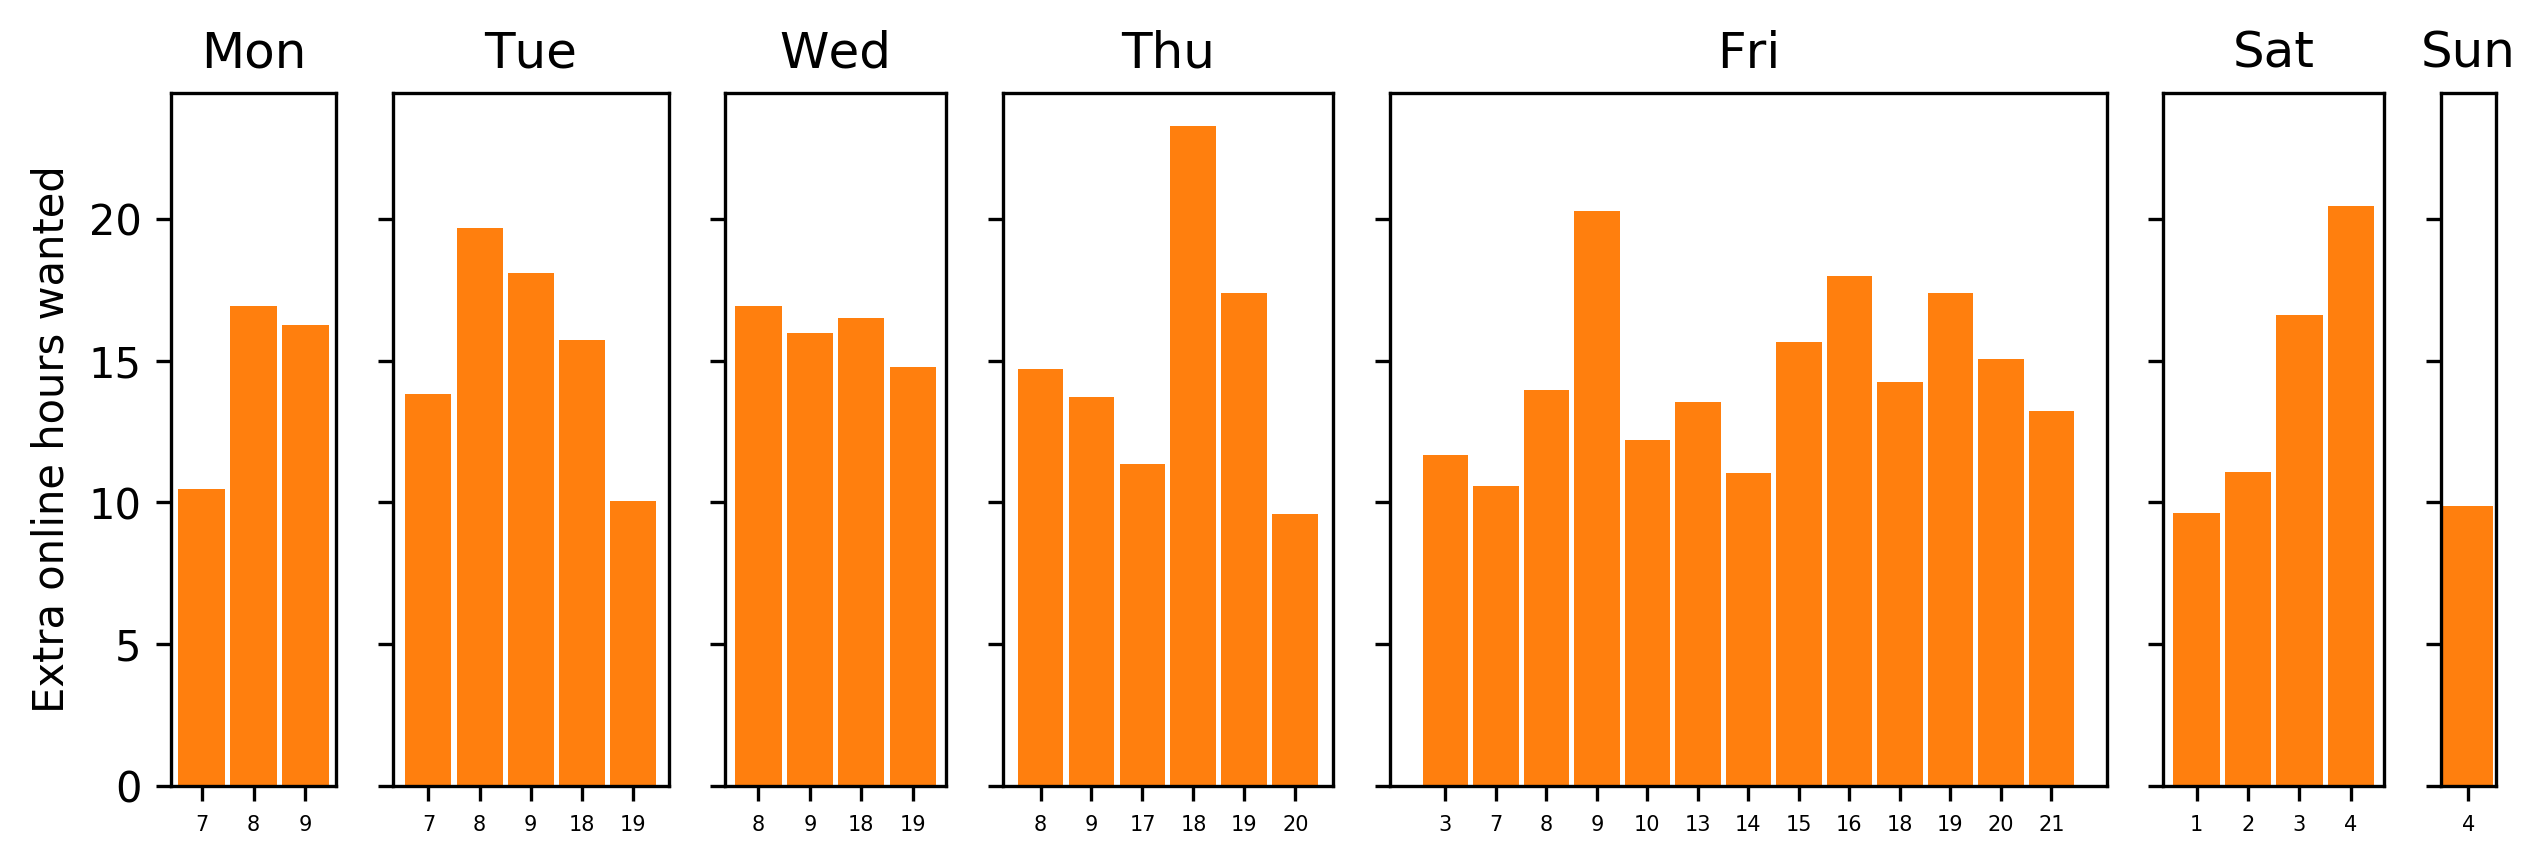
\includegraphics[width=\textwidth]{task4/extra_hours}
    \end{center}
    
    
    %%%%%%%%%%%%%%%%%%%%%%%%%%%%%%%%%%%%%%%%%%%%%%%%%%
    \section{Levels of guaranteed hourly earnings}
    %%%%%%%%%%%%%%%%%%%%%%%%%%%%%%%%%%%%%%%%%%%%%%%%%%
    
    (Unclear)
    
    
    %%%%%%%%%%%%%%%%%%%%%%%%%%%%%%%%%%%%%%%%%%%%%%%%%%
    \section*{Code}
    %%%%%%%%%%%%%%%%%%%%%%%%%%%%%%%%%%%%%%%%%%%%%%%%%%
    
    The code is at
    \begin{center}
        \url{https://github.com/numpde/misc/tree/master/homeworks/bolt}
    \end{center}

\end{document}
